%https://tex.stackexchange.com/questions/411920/labels-on-a-grouped-and-stacked-bar-chart
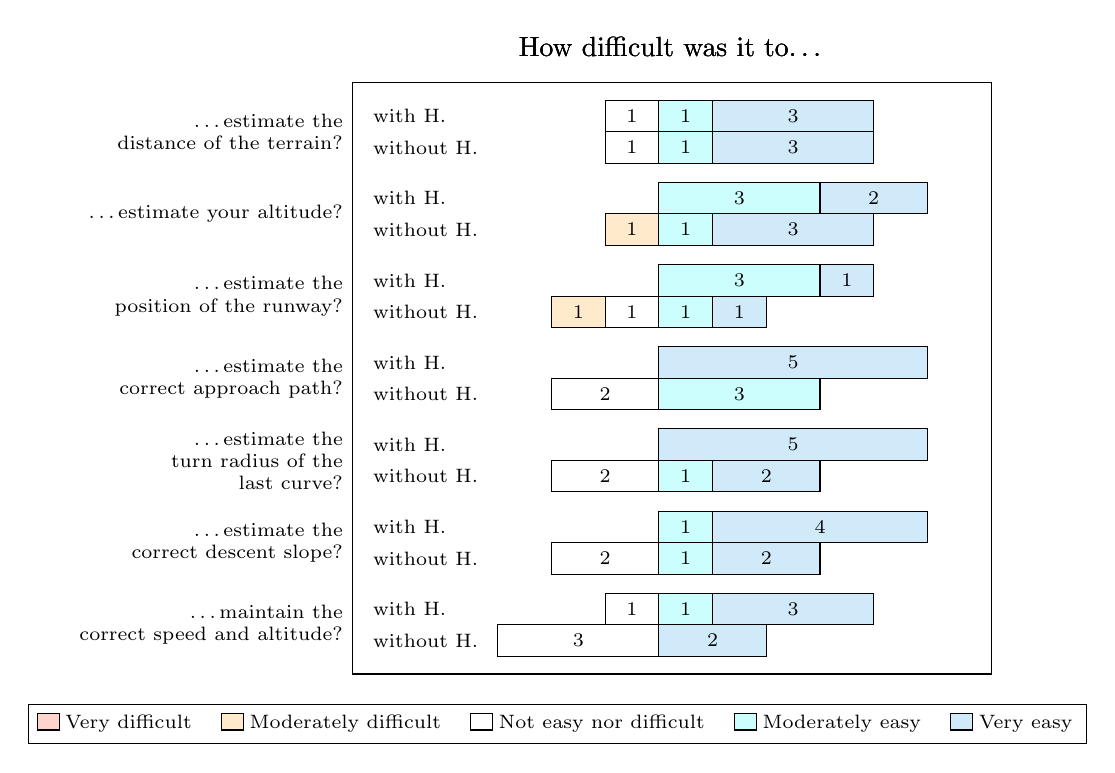
\begin{tikzpicture}[
    %every node/.style=draw,
    %every label/.style=draw
]
    \definecolor{myred}{RGB}{218,32,0}
    \definecolor{myredfill}{RGB}{255,212,204}
    \definecolor{myorange}{RGB}{255,153,0}
    \definecolor{myorangefill}{RGB}{255,235,204}
    \definecolor{mygreen}{RGB}{0,184,0}
    \definecolor{mygreenfill}{RGB}{202,255,202}
    \definecolor{mycyan}{RGB}{5,154,199}
    \definecolor{mycyanfill}{RGB}{205,254,254}
    \definecolor{myblue}{RGB}{13,98,153}
    \definecolor{mybluefill}{RGB}{208,234,250}

    \pgfplotsset{
        every axis/.style={
            xbar stacked,
            width=0.8\textwidth,
            height=0.75\textwidth,
            bar width=4mm,
            title={How difficult was it to\ldots},
            %symbolic y coords = {Q1,Q2,Q3},
            ytick = {0, 1, 2, 3, 4, 5, 6},
            yticklabels = {
                \ldots maintain the\\correct speed and altitude?,
                \ldots estimate the\\correct descent slope?,
                \ldots estimate the\\turn radius of the\\last curve?,
                \ldots estimate the\\correct approach path?,
                \ldots estimate the\\position of the runway?,
                \ldots estimate your altitude?,
                \ldots estimate the\\distance of the terrain?
            },
            yticklabel style={font=\scriptsize, align=right},
            ytick style = {draw = none},
            xtick = \empty,
            xmin=-4, xmax=4.5,
            enlarge y limits=0.1,
            enlarge x limits=0.2,
            legend style={
                at={(0.32,-0.05)},
                anchor=north,
                legend columns=5,
                /tikz/every even column/.append style={column sep=0.3cm},
                font=\scriptsize
            },
            nodes near coords,
            nodes near coords style={font=\scriptsize, align=center},
            point meta=explicit symbolic,
            % extra x ticks={0},
            % extra x tick style={
            %     grid style={black},
            %     xticklabel=\empty,
            % },
        }    
    }

    \begin{axis}[bar shift = 2mm, yticklabels={}]
        \addplot+[xbar, black, fill=white] plot coordinates {
            (-1,6) [1]
            (0,5) [0]
            (0,4) [0]
            (0,3) [0]
            (0,2) [0]
            (0,1) [0]
            (-1,0) [1]
        };
        \addplot+[xbar, black, fill=myorangefill] plot coordinates {
            (0,6) [0]
            (0,5) [0]
            (0,4) [0]
            (0,3) [0]
            (0,2) [0]
            (0,1) [0]
            (0,0) [0]
        };
        \addplot+[xbar, black, fill=myredfill] plot coordinates {
            (0,6) [0]
            (0,5) [0]
            (0,4) [0]
            (0,3) [0]
            (0,2) [0]
            (0,1) [0]
            (0,0) [0]
        };
        \addplot+[xbar, black, fill=mycyanfill] plot coordinates {
            (1,6) [1]
            (3,5) [3]
            (3,4) [3]
            (0,3) [0]
            (0,2) [0]
            (1,1) [1]
            (1,0) [1]
        };
        \addplot+[xbar, black, fill=mybluefill] plot coordinates {
            (3,6) [3]
            (2,5) [2]
            (1,4) [1]
            (5,3) [5]
            (5,2) [5]
            (4,1) [4]
            (3,0) [3]
        };

        \node[right,yshift=2mm] at (-5.5, 0) {\scriptsize with H.};
        \node[right,yshift=2mm] at (-5.5, 1) {\scriptsize with H.};
        \node[right,yshift=2mm] at (-5.5, 2) {\scriptsize with H.};
        \node[right,yshift=2mm] at (-5.5, 3) {\scriptsize with H.};
        \node[right,yshift=2mm] at (-5.5, 4) {\scriptsize with H.};
        \node[right,yshift=2mm] at (-5.5, 5) {\scriptsize with H.};
        \node[right,yshift=2mm] at (-5.5, 6) {\scriptsize with H.};
    \end{axis}

    \begin{axis}[bar shift = -2mm]
        \addplot+[xbar, black, fill=myredfill] plot coordinates {
            (0,6) [0]
            (0,5) [0]
            (0,4) [0]
            (0,3) [0]
            (0,2) [0]
            (0,1) [0]
            (0,0) [0]
        };
        \addplot+[xbar, black, fill=white] plot coordinates {
            (-1,6) [1]
            (0,5) [0]
            (-1,4) [1]
            (-2,3) [2]
            (-2,2) [2]
            (-2,1) [2]
            (-3,0) [3]
        };
        \addplot+[xbar, black, fill=myorangefill] plot coordinates {
            (0,6) [0]
            (-1,5) [1]
            (-1,4) [1]
            (0,3) [0]
            (0,2) [0]
            (0,1) [0]
            (0,0) [0]
        };
        \addplot+[xbar, black, fill=mycyanfill] plot coordinates {
            (1,6) [1]
            (1,5) [1]
            (1,4) [1]
            (3,3) [3]
            (1,2) [1]
            (1,1) [1]
            (0,0) [0]
        };
        \addplot+[xbar, black, fill=mybluefill] plot coordinates {
            (3,6) [3]
            (3,5) [3]
            (1,4) [1]
            (0,3) [0]
            (2,2) [2]
            (2,1) [2]
            (2,0) [2]
        };
        \node[right,yshift=-2mm] at (-5.5, 0) {\scriptsize without H.};
        \node[right,yshift=-2mm] at (-5.5, 1) {\scriptsize without H.};
        \node[right,yshift=-2mm] at (-5.5, 2) {\scriptsize without H.};
        \node[right,yshift=-2mm] at (-5.5, 3) {\scriptsize without H.};
        \node[right,yshift=-2mm] at (-5.5, 4) {\scriptsize without H.};
        \node[right,yshift=-2mm] at (-5.5, 5) {\scriptsize without H.};
        \node[right,yshift=-2mm] at (-5.5, 6) {\scriptsize without H.};
        %\legend{Very difficult, Not easy nor difficult, Moderately difficult, Moderately easy, Very easy}
    \end{axis}

    \begin{axis}[ytick = \empty]
        \addplot+[xbar, black, fill=myredfill] plot coordinates {
            (0,0) [0]
        };
        \addplot+[xbar, black, fill=myorangefill] plot coordinates {
            (0,0) [0]
        };
        \addplot+[xbar, black, fill=white] plot coordinates {
            (0,0) [0]
        };
        \addplot+[xbar, black, fill=mycyanfill] plot coordinates {
            (0,0) [0]
        };
        \addplot+[xbar, black, fill=mybluefill] plot coordinates {
            (0,0) [0]
        };
        \legend{Very difficult, Moderately difficult, Not easy nor difficult, Moderately easy, Very easy}
    \end{axis}


\end{tikzpicture}